\documentclass[../main.tex]{subfiles}

\begin{document}

\subsection{Overview: High-level components and their interaction}
 TrackMe will be developed on a 3-tier architecture (\textit{Fig. 1}), the rationale behind application servers separation
 is to mantain Data4Help service aimed at companies, independent from AutomatedSOS and Track4Run functionalities, aimed at users.
 Application servers will interact with a database server.
 Adding the tier 2 will provide services separation and will  make possible to handle failures and updates without the whole system going down.


\begin{figure}[ht]
\centering
     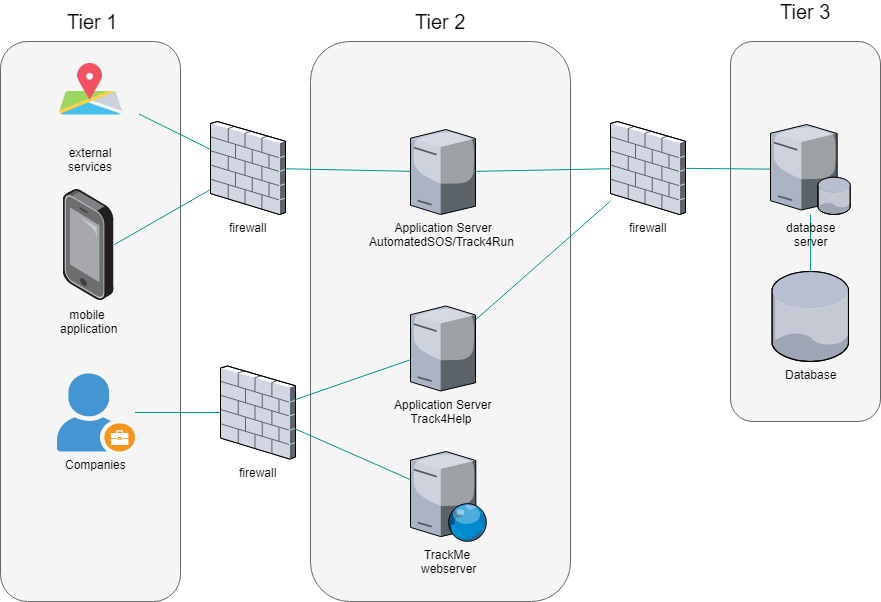
\includegraphics[width=1.0\textwidth]{trackme_architecture.png}
      \caption{TrackMe architecture}
       \label{fig:trackme_architecture}
\end{figure}

\begin{figure}[ht]
    \centering
         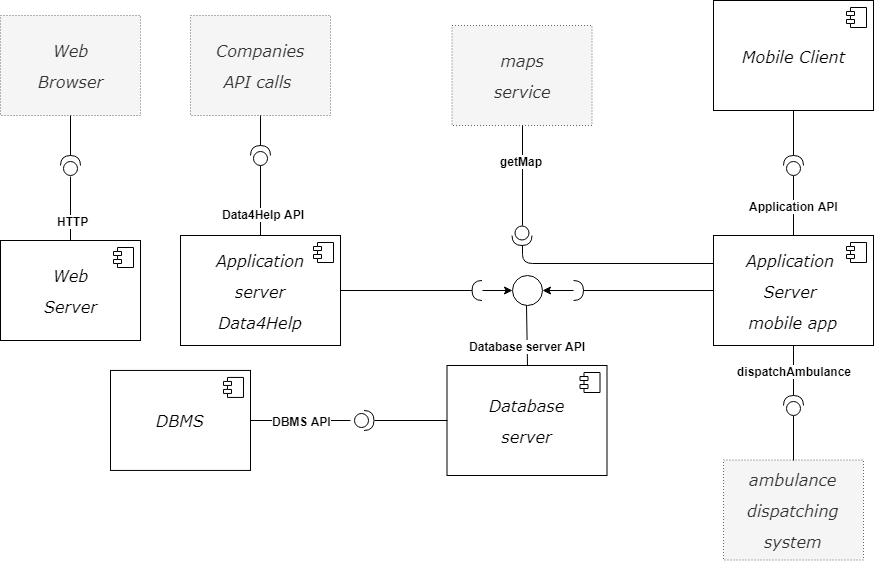
\includegraphics[width=1.0\textwidth]{high_level_component.png}
          \caption{High level components view}
           \label{fig:high_level_components}
\end{figure}

\newpage
\subsection{Component view}
\begin{figure}[H]
	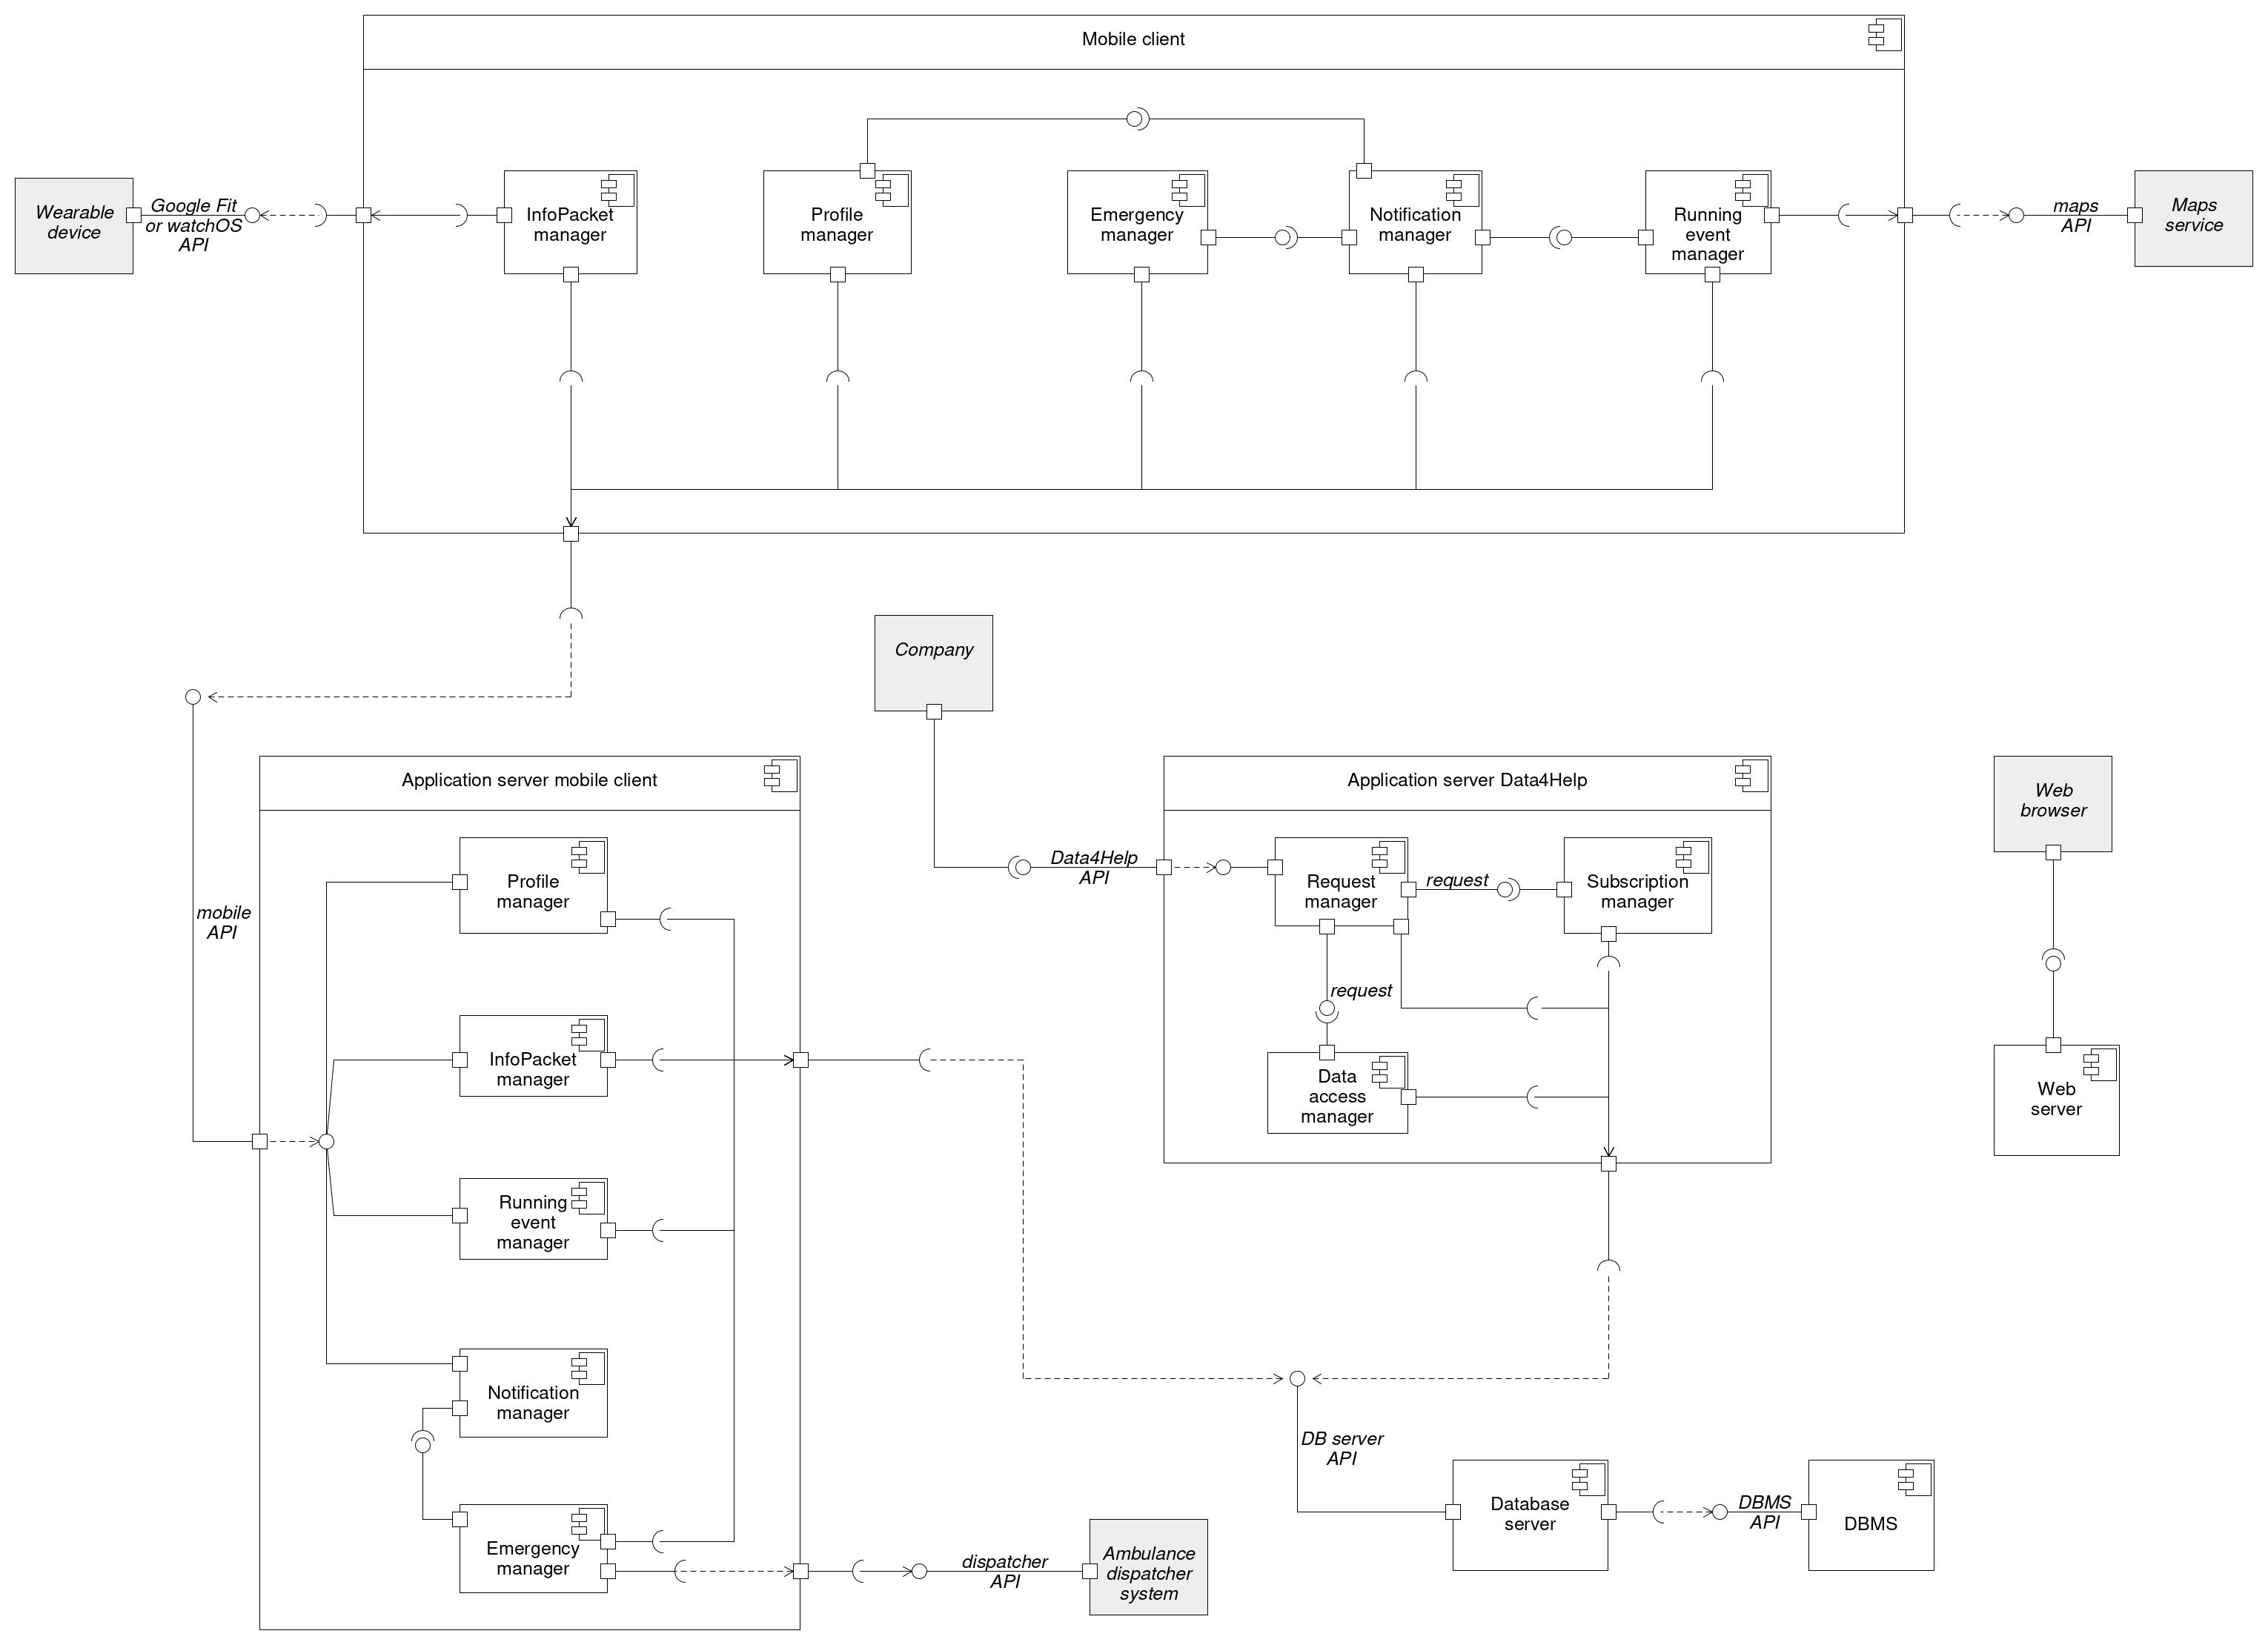
\includegraphics[width=\paperwidth, angle=90]{uml_component_view.jpg}
	\caption{Component view}
	\label{fig:uml_component_view}
\end{figure}
\newpage

\subsubsection{Mobile client} This is the mobile application. It will be built on top of the mobile platform's specific API, not represented in this diagram, and dependent on the wearable device's API (Google Fit or watchOS) and on the maps service provider's API for Track4Run functionalities. Moreover, it will communicate with the REST server, the Application server mobile client component, through HTTPS protocol, using the REST API the component will provide.

\begin{description}

	\item{\bf Profile manager} This component will handle all functionalities regarding the user, such as registration, login, registering a new wearable device or removing a registered one, changing the preferences, accepting or refusing specific data requests sent from a company, and the activation or deactivation of AutomatedSOS and Track4Run services.

	\item{\bf InfoPacket manager} This is the component in charge of periodically getting the body parameters from a wearable device and location coordinates, and sending them to the Application server mobile client component.

	\item{\bf Emergency manager} This component is part of the AutomatedSOS service: it will handle an emergency situation, displaying useful information on the screen.

	\item{\bf Running event manager} This component is part of the Track4Run service: it will allow the user to create a new event, view the available events near his/her position, and enroll into them. It will also let the user view informations about an event in progress, like the position of the runners on a map.

	\item{\bf Notification manager} This component will simply display notification to the user when such is received from the server, such as a new specific request for data.

\end{description}

%TODO rework%
\subsubsection{Application server mobile client}  This is the REST server that will interact with the mobile client, and will forward every information received from it to the Database server component to store them. It will expose various REST endpoints to handle every action received from the mobile client; for this reason, its composition is very similar to the one found in the mobile client component. However the implementation of the interfaces used will be different: for example, the Emergency handler component, in this case, will interact with the external Ambulance dispatcher system through its API to dispatch and ambulance to the user's location.

\subsubsection{Application server Data4Help} This is the REST server aimed to be used from companies. It will let them make requests for data, for a group of users or for a specific user, and subscribe for new informations.

\begin{description}

	\item{\bf Request manager} This component will handle the data requests received from companies: through the help of the Data access manager component, will determine if the company can have access to such user's data, in case of a group request, or will register the request in case it's a specific one, and then eventually will send the data to the company as a response.

	\item{\bf Subscription manager} This component will handle the subscriptions a company may have, sending the data from the users to the company as soon as it's received.

	\item{\bf Data access manager} This component will determine if a company can have access to some data, after it has made a request for it. In particular, will count how many users satisfy a group request and authorize or reject it based on this number, and will also regulate the access to users data every request grants.

\end{description}

\subsubsection{Database server} This is server is the only component that have access to the DBMS. Every other component will interact with the API this component makes available to read and write on the database. This allows the other components to be independent from the specific implementation of the database controller that will directly interact with the database, providing the ability to change how the system interfaces to the DBMS without altering all the components mentioned above.
                                Moreover this design gives a further layer of security making the system resilient to a possible \textit{CIA} security violation 

\subsubsection{Web server} This component will be a static server offering information about TrackMe and documentation on our APIs for third party companies. Also, as stated in the RASD, it will offer a form for companies to register on our service and request an API key.

\subsection{Deployment view}

\begin{figure}[H]
        \centering
             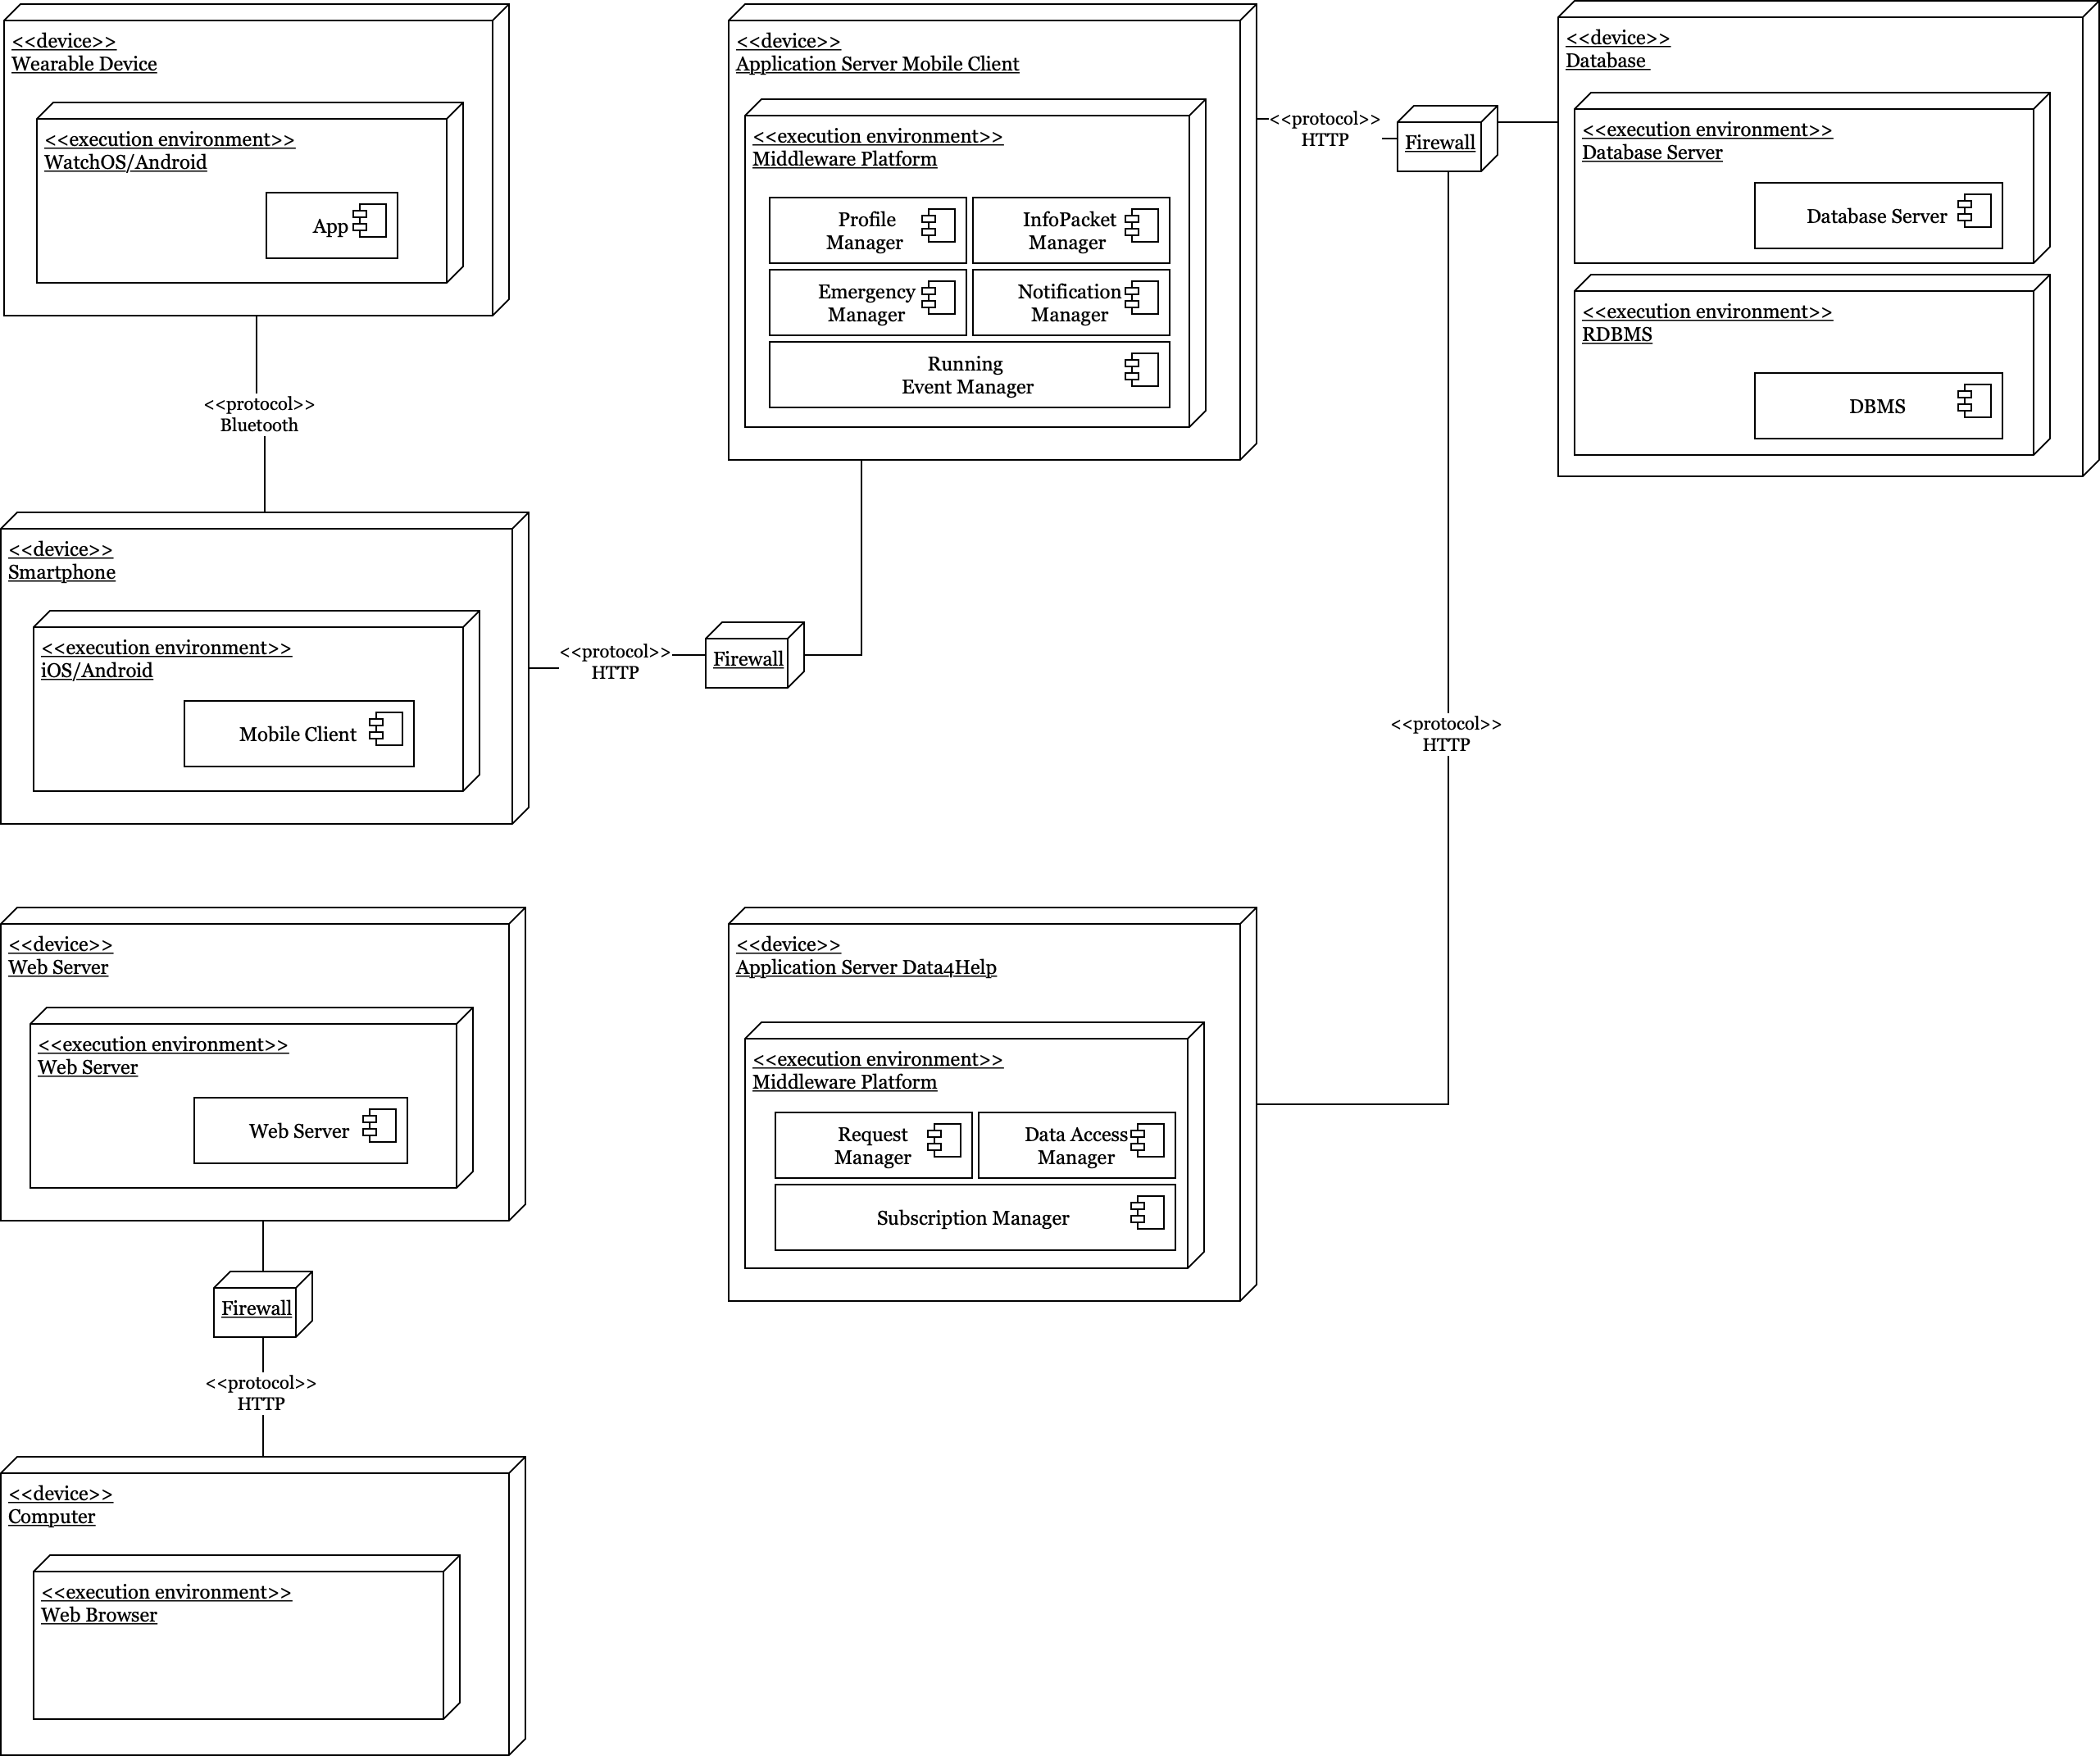
\includegraphics[width=1.0\textwidth]{deploymentView.png}
              \caption{Deployment Diagram }
               \label{fig:deploymentView}
\end{figure}

\newpage

\subsection{Runtime view}
In this section are shown the sequence diagrams of some features. They are useful to clarify the runtime behaviour of the components involved for each functionality.
\begin{figure}[H]
        \centering
             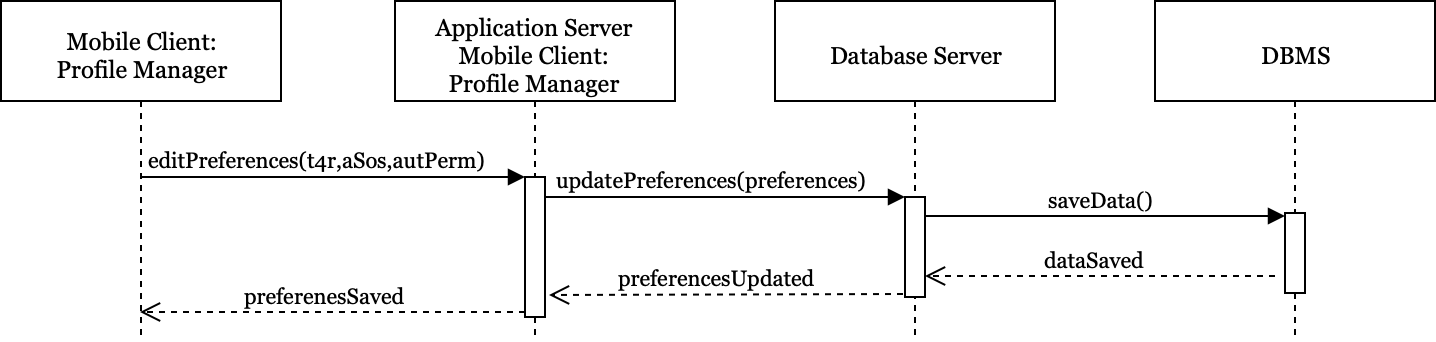
\includegraphics[width=1.0\textwidth]{editPreferencesSD.png}
              \caption{Sequence Diagram Edit Preferences }
               \label{fig:editPreferencesSD}
\end{figure}

\vspace*{2cm}

\begin{figure}[H]
        \centering
             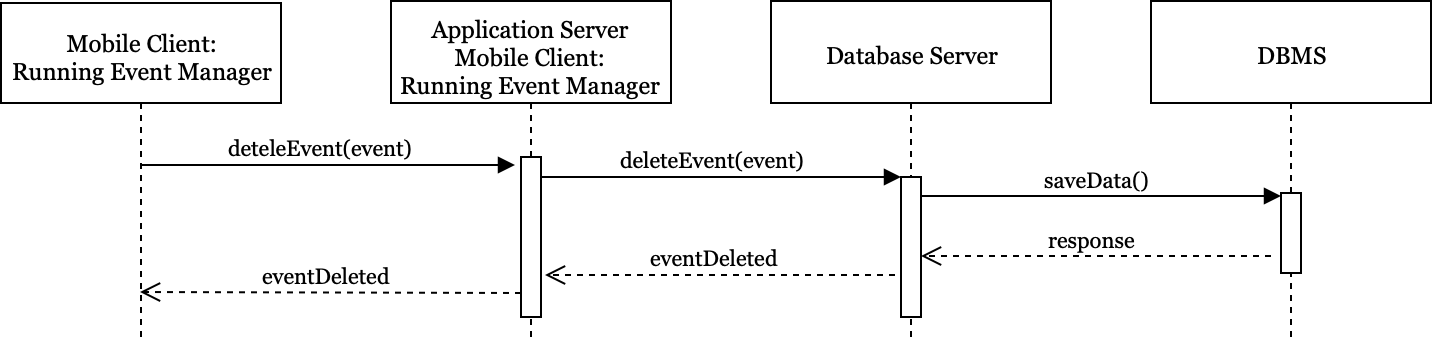
\includegraphics[width=1.0\textwidth]{deleteRunningEventSD.png}
              \caption{Sequence Diagram Delete Running Event }
               \label{fig:deleteRunningEventSD}
\end{figure}

\vspace*{2cm}

\begin{figure}[H]
        \centering
             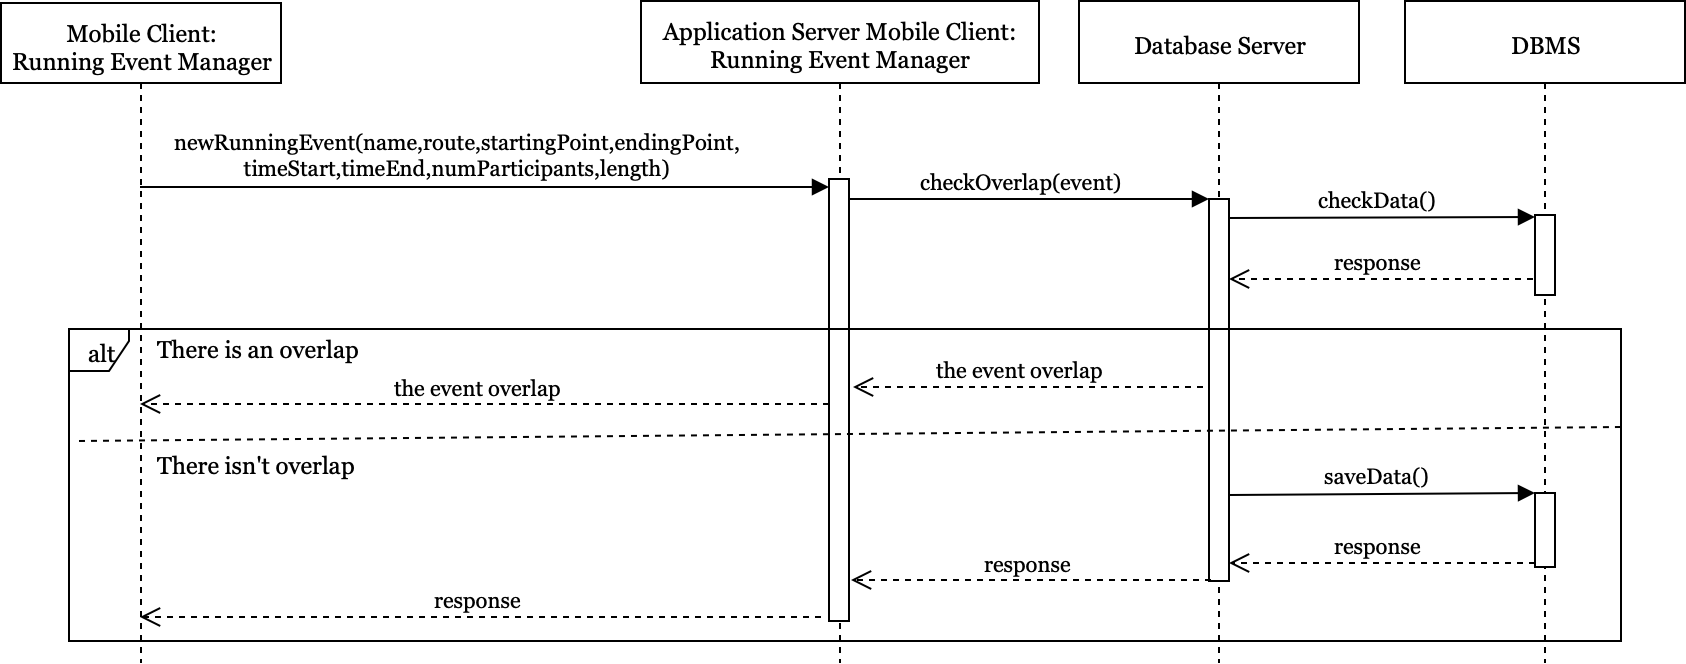
\includegraphics[width=1.0\textwidth]{createRunningEventSD.png}
              \caption{Sequence Diagram Create Running Event }
               \label{fig:createRunningEventSD}
\end{figure}

\vspace*{2cm}

\begin{figure}[H]
        \centering
             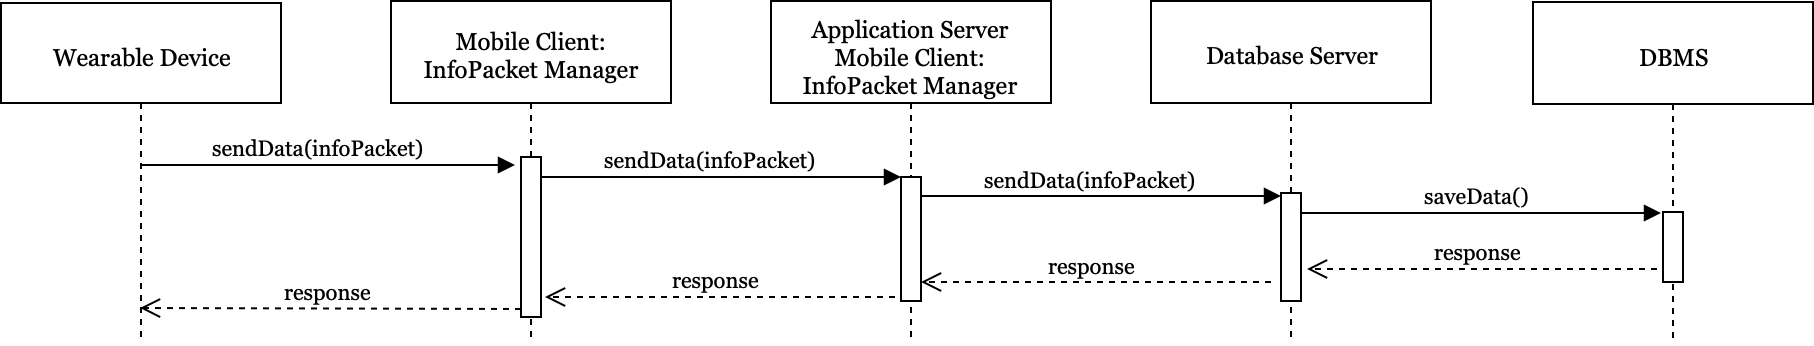
\includegraphics[width=1.0\textwidth]{data4HelpSD.png}
              \caption{Sequence Diagram Data4Help Service }
               \label{fig:data4HelpSD}
\end{figure}

\vspace*{2cm}

\begin{figure}[H]
        \centering
             \includegraphics[width=1.0\textwidth]{data4HelpNotificationSD.png}
              \caption{Sequence Diagram Data4Help Notification  }
               \label{fig:data4HelpSD}
\end{figure}

\vspace*{2cm}

\begin{figure}[H]
        \centering
             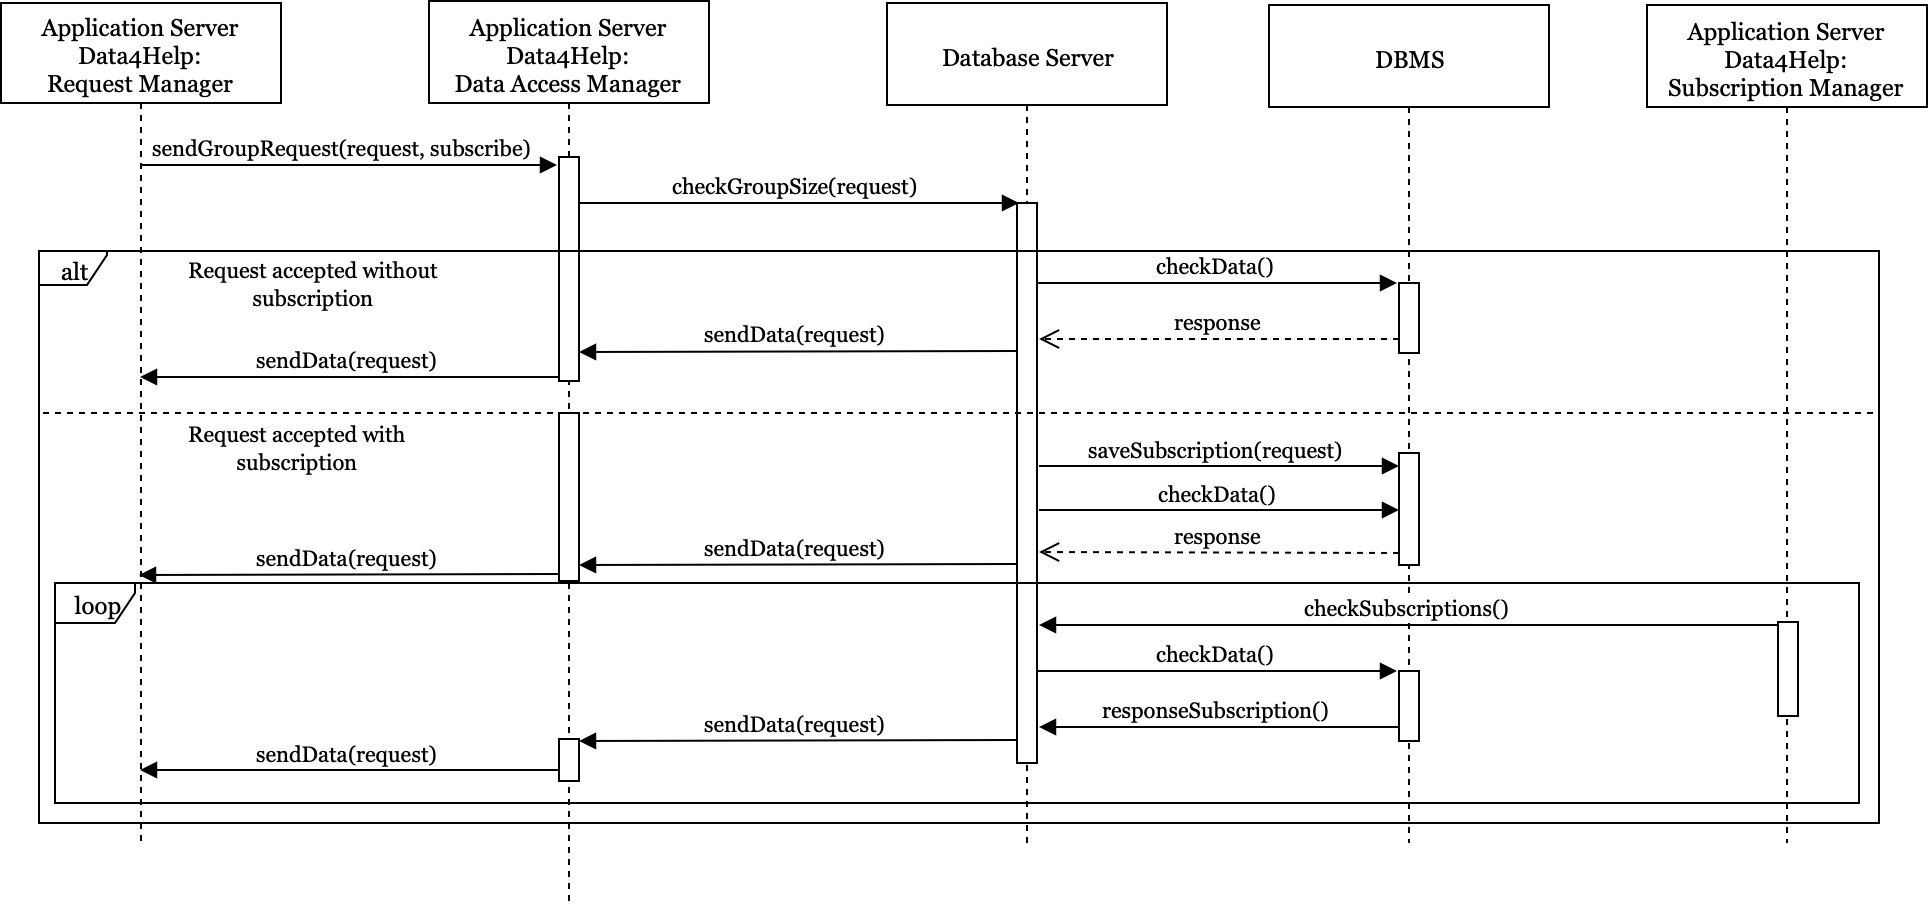
\includegraphics[width=1.0\textwidth]{data4HelpRequestSD.png}
              \caption{Sequence Diagram Data4Help Group Request Service }
               \label{fig:data4HelpRequestSD}
\end{figure}

\vspace*{2cm}

\begin{figure}[H]
        \centering
             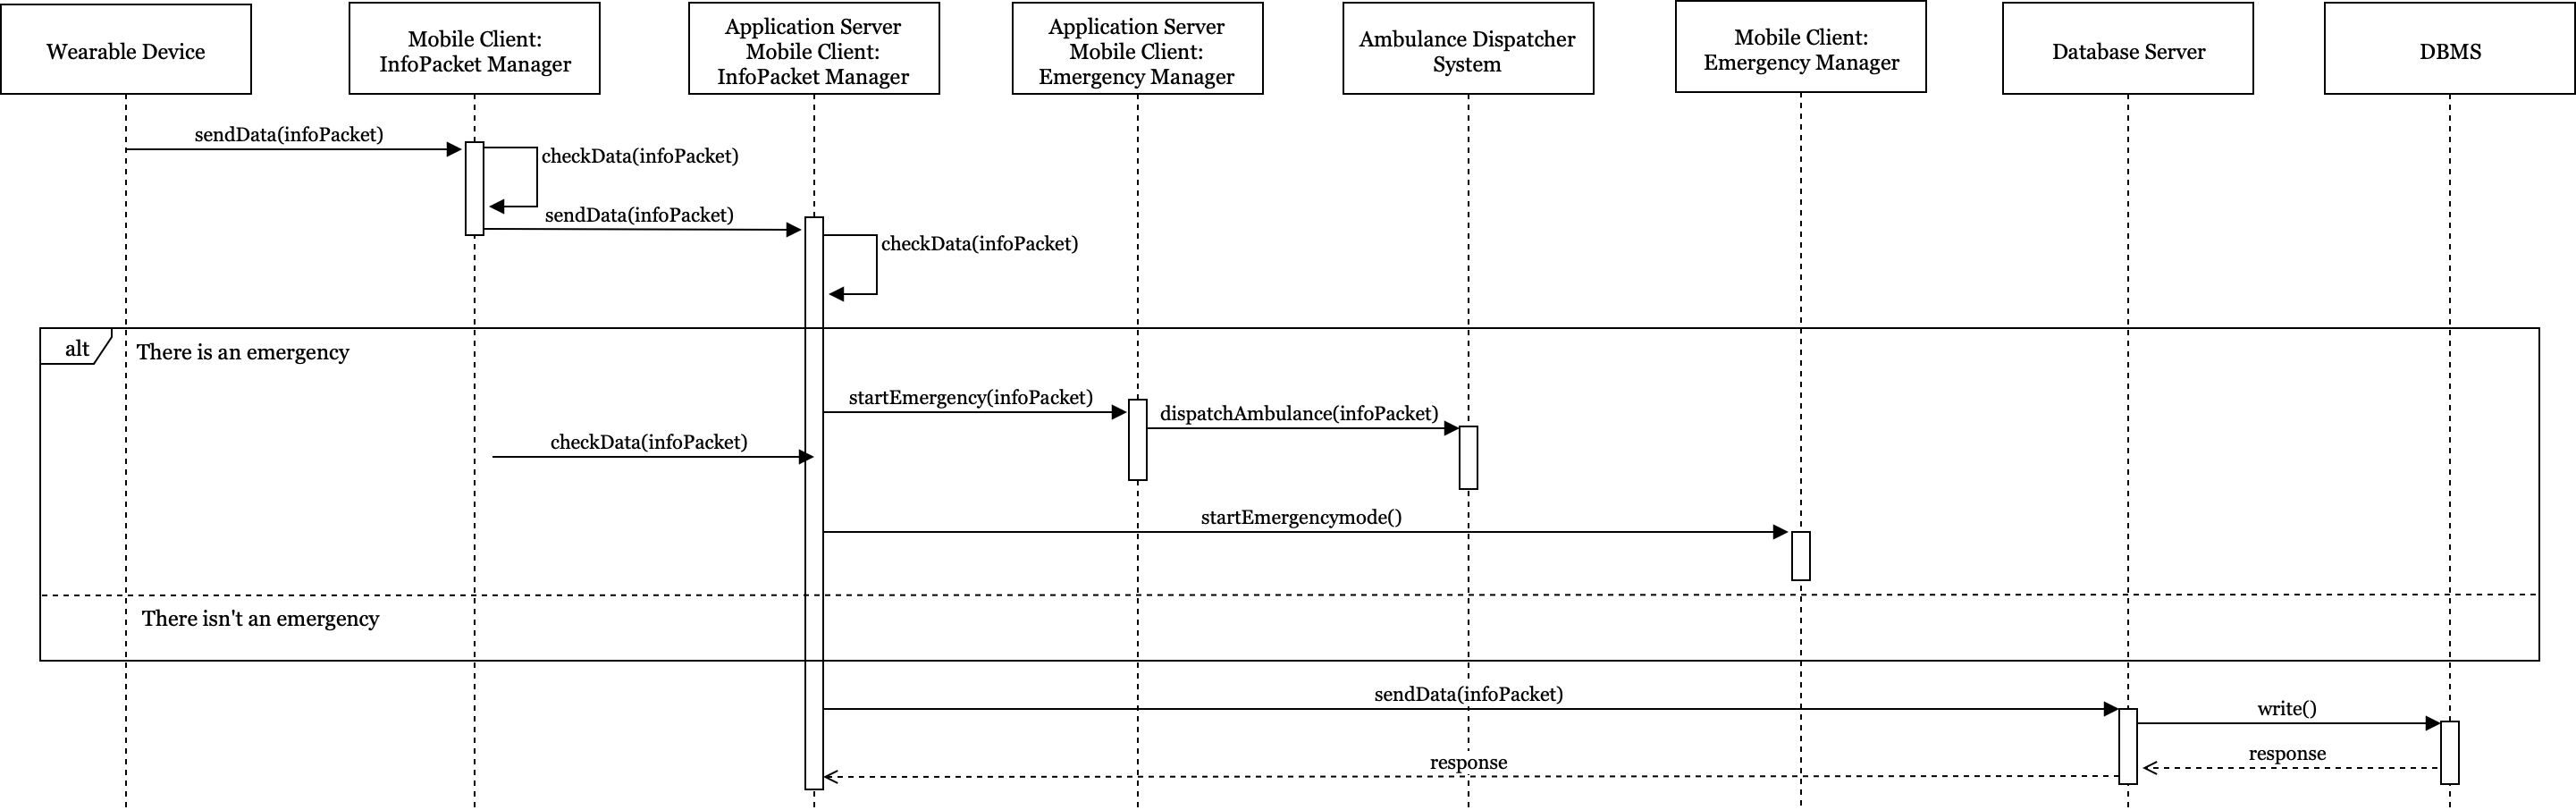
\includegraphics[width=1.0\textwidth]{ambulanceDispatchingSD.png}
              \caption{Sequence Diagram AutomatedSOS Service Dispatching Ambulance}
               \label{fig:ambulanceDispatchingSD}
\end{figure}

\subsection{Component interfaces}

In this chapter are listed all interfaces that permit to the various components to communicate.

In the Application server components, the APIs exposed are composed of various interfaces that handle the appropriate functions.

Not represented here is the DB Server API, exposed by the Database server component, which is composed of all the functions necessary for the other components to interact with the DBMS.

\begin{figure}[H]
        \centering
             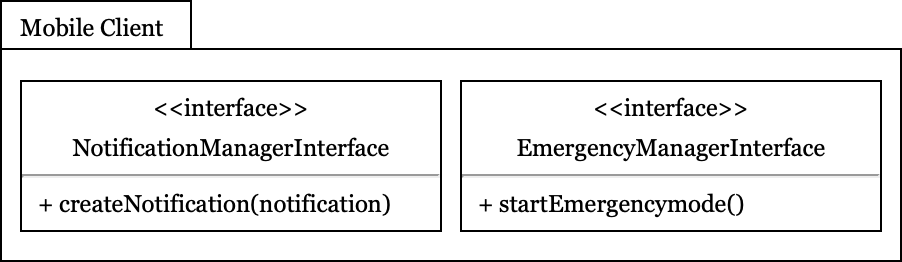
\includegraphics[width=0.75\textwidth]{componentInterfacesMobileClient.png}
              \caption{Component Interfaces Mobile Client }
               \label{fig:componentInterfacesMobileClient}
\end{figure}

\vspace*{2cm}

\begin{figure}[H]
        \centering
             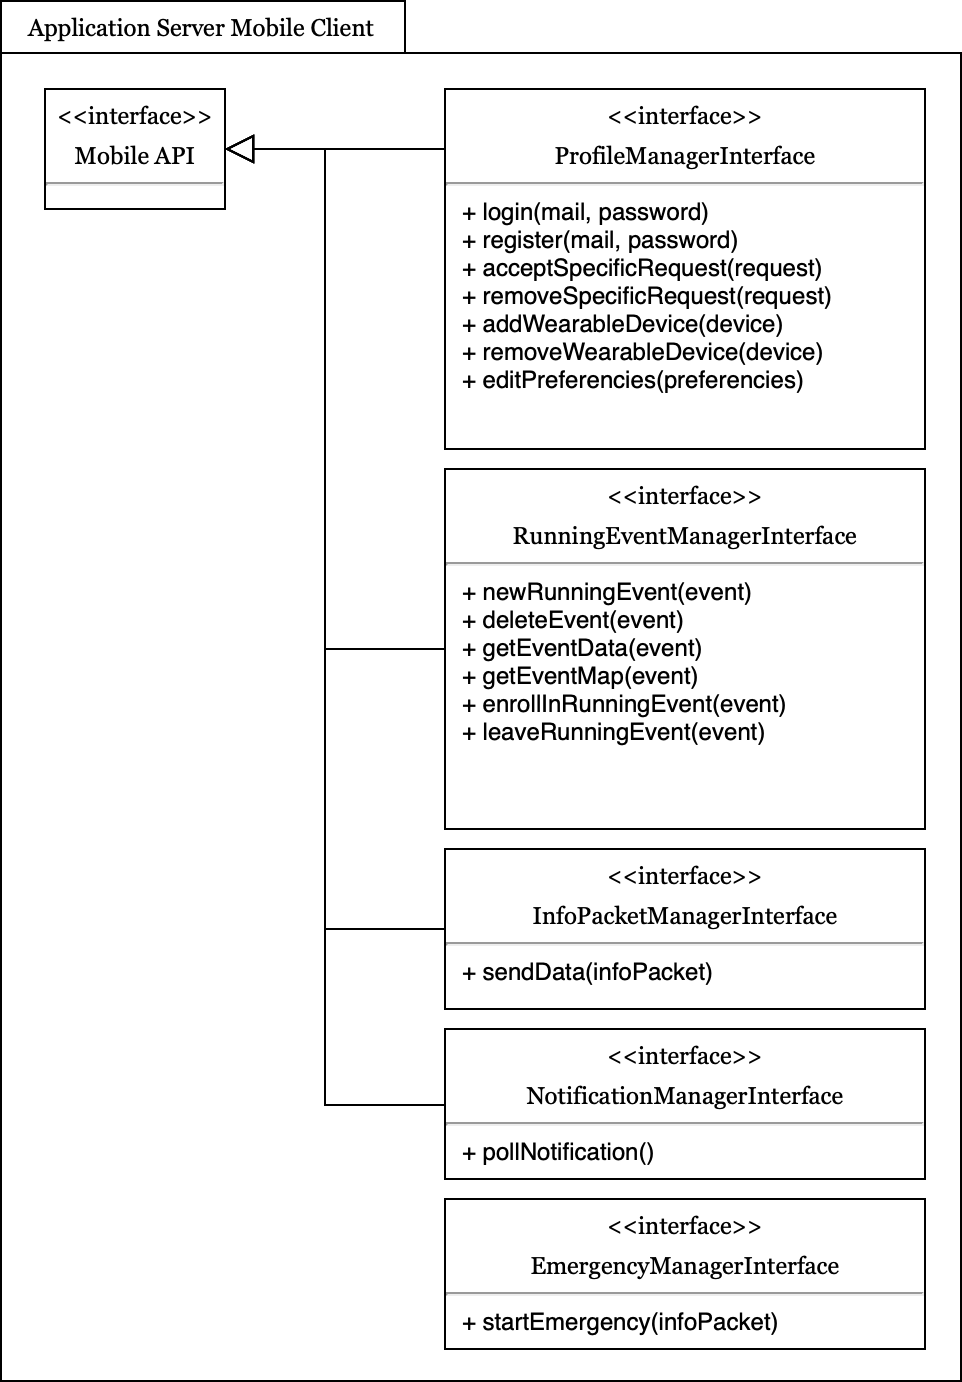
\includegraphics[width=0.75\textwidth]{componentInterfacesAppServerMobClient.png}
              \caption{Component Interfaces Application Server Mobile Client}
               \label{fig:componentInterfacesAppServerMobClient}
\end{figure}

\vspace*{2cm}

\begin{figure}[H]
        \centering
             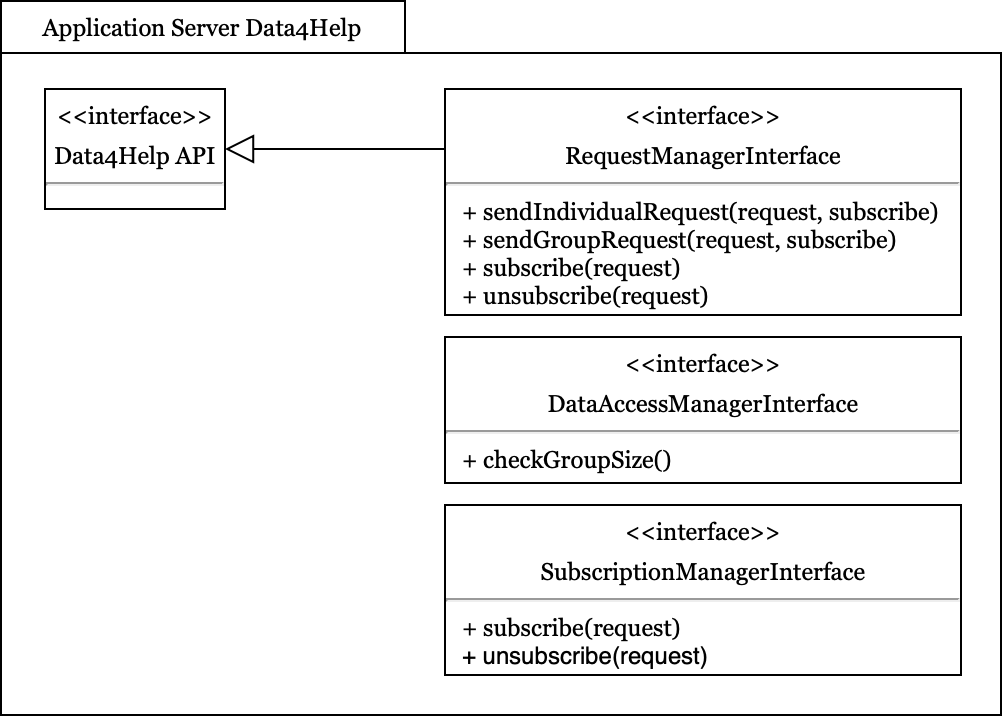
\includegraphics[width=0.75\textwidth]{componentInterfacesAppServerD4H.png}
              \caption{Component Interfaces Application Server Data4Help }
               \label{fig:componentInterfacesAppServerD4H}
\end{figure}

\vspace*{2cm}


\subsection{Selected architectural styles and patterns}

A client-server model will be followed the mobile application, while the part of the system that is oriented towards third party companies will be composed only by a server exposing them the useful APIs. All servers will be RESTful:
\begin{itemize}
	\item The endpoints, i.e. the APIs they expose, will have meaningful URIs, pertient to the function they serve.
	\item The communication will rely on HTTP status codes and, when needed, error messages in the HTTP body for informing a successfull or unsuccessful operation.
	\item The interaction with them will follow the CRUD paradign to perform any operation.
\end{itemize}

This design allows for an event driven and resource centric system that is especially performant in managing a large number of customer interactions simultaneously (eg. frequently collected user's parameters).

\subsection{Other design decisions}

\begin{description}
	\item Registration and login functionality for end users will make use of HTTP basic authentication. The passwords shall be stored as hashes on the database following security best practices.
	\item All HTTP traffic shall be encapsulated through SSL to preserve confidentiality.
	\item Every registered company will have a unique authorized by TrackMe APIkey to make REST requests.
\end{description}

\end{document}
